%%%%%%%%%%%%%%%%%%%%%%%%%%%%%%%%%%%%%%%%%%%%%%%
% Design and Cryptanalysis of a Customizable
% Authenticated Encryption Algorithm
% 
% A Master's Thesis Defense
%
% Author: Matt Kelly (mjk7841@rit.edu)
% Defended: August 1, 2014
%
% Thesis document available at:
% github.com/mattkelly/masters-thesis
%%%%%%%%%%%%%%%%%%%%%%%%%%%%%%%%%%%%%%%%%%%%%%%
\documentclass[11pt,american]{beamer}
%\usefonttheme[onlymath]{serif}
\usepackage[utf8]{inputenc}
\usepackage{url}
\usepackage{subfigure}
\usepackage{babel}
\usepackage{times}
\usepackage{graphicx}
\usepackage{amsmath}
\usepackage{amssymb}
\usepackage{verbatim}
\usepackage{enumerate}
\usepackage{afterpage}
\usepackage[mathscr]{euscript}
\usepackage{xcolor}   % For colored links
\usepackage{hyperref} % For internal links
\usepackage{nag}      % Warn about old packages and commands
\usepackage{fixltx2e} % Fix misc. LaTeX stuff
\usepackage{xspace}   % Fix spacing at end of macros
\usepackage{array}
\usepackage{etoolbox}
\usepackage{multirow}
\usepackage{rotating}
\usepackage{listings}

\usepackage{tikz}
\usetikzlibrary{calc}

\setbeamertemplate{bibliography item}{[\theenumiv]}

\lstset{%
  basicstyle=\tiny,
  frame=single
}

\setcounter{MaxMatrixCols}{16}

\newenvironment{smallpmatrix}
  {\left(\begin{smallmatrix}}
  {\end{smallmatrix}\right)}

% For now, to help organize
\setcounter{tocdepth}{5}
\newcommand{\TODO}{\textcolor{red}{\textbf{TODO}}\xspace}

\usepackage{verbatim} % For block comments
\usepackage{amssymb}  % http://ctan.org/pkg/amssymb
\usepackage{pifont}   % http://ctan.org/pkg/pifont
\usepackage{graphicx} % For images
\usepackage{booktabs} % \toprule, \midrule, \bottomrule
\usepackage{nag}      % Warn about old packages and commands
\usepackage{fixltx2e} % Fix misc. LaTeX stuff
\usepackage{multirow}
\usepackage{rotating} 
\usepackage{listings} % Code listings
\usepackage{xspace}   % Fix spacing at end of macros
\usepackage{array}
\usepackage{etoolbox}
\usepackage{lscape}
\usepackage{verbatim}
\usepackage{enumerate}

\usepackage{tikz}
\usetikzlibrary{calc}

\mode<presentation> {
  \usetheme{CambridgeUS}
  % Remove navigation symbols from slides
  \setbeamertemplate{navigation symbols}{}
}

%\newcommand{\cmk}{\color{green}\ding{51}} % Check mark
%\newcommand{\xmk}{\color{red}\ding{55}}   % X mark

\newcommand{\Ztwo}{\ensuremath{\mathbb{Z}_2}\xspace}
\newcommand{\Zn}{\ensuremath{\mathbb{Z}_n}\xspace}
\newcommand{\gftwo}{\ensuremath{\mathrm{GF}(2)}\xspace}
\newcommand{\gfsixteen}{\ensuremath{\mathrm{GF}(2^{16})}\xspace}
\newcommand{\ourpoly}{\ensuremath{x^{16} + x^5 + x^3 + x^2 + 1}\xspace}
\newcommand{\gfwithpoly}{\ensuremath{\text{GF}(2^{16}) / \left\langle \ourpoly \right\rangle}\xspace}

%\newcommand{\pval}{\ensuretext{P\text{-}value}\xspace}
%\newcommand{\pvals}{\ensuretext{P\text{-}values}\xspace}
\newcommand{\pval}{\textit{P-value}\xspace}
\newcommand{\pvals}{\textit{P-values}\xspace}

\newcommand{\Keccak}{\textsc{Keccak}\xspace}
\newcommand{\SpongeWrap}{\textsc{SpongeWrap}\xspace}

\newcommand{\drawxTimes}[2]{% center: x,y
  \draw[fill=gray!15,line width=2.5pt] (#1, #2) ellipse (1em and 1em) node {$x*$};
}
\newcommand{\drawXOR}[2]{% center: x,y
  \draw[fill=gray!15,line width=2.5pt] (#1, #2) ellipse (1em and 1em);
  \draw[line width=2.5pt] (#1-.4, #2) -- (#1+.4, #2);
  \draw[line width=2.5pt] (#1, #2-.4) -- (#1, #2+.4);
}
\newcommand{\drawAdder}[2]{% top left: x,y
  \draw[fill=gray!15,line width=2.5pt] (#1, #2) rectangle (#1+1, #2-1);
  \draw[line width=2.5pt] (#1, #2-.5) -- (#1+1, #2-.5);
  \draw[line width=2.5pt] (#1+.5, #2-1) -- (#1+.5, #2);
}
\newcommand{\drawRot}[2]{% center: x,y
  \draw[fill=gray!15,line width=2.5pt] (#1, #2) ellipse (2em and 1em) node {$\mathbf{ROT}$};
}
\newcommand{\drawMixerInputs}{
  \draw[fill=gray!30] (0,16) rectangle (2,15) node[midway] {$A$};
  \draw[fill=gray!30] (4,16) rectangle (6,15) node[midway] {$B$};
}
\newcommand{\drawMixerOutputs}[1]{%y offset from top
  \draw[fill=gray!30] (0,16-#1) rectangle (2,15-#1) node[midway] {$A'$};
  \draw[fill=gray!30] (4,16-#1) rectangle (6,15-#1) node[midway] {$B'$};
}

% Aliases for readability
\let\from=\colon
\let\to=\rightarrow

% The short title appears at the bottom of every slide, the full title is only on the title page
\title[Customizable AE Algorithm]
{Design and Cryptanalysis of a Customizable Authenticated Encryption Algorithm}
\subtitle{A Master's Thesis Defense}

\author{Matthew J. Kelly} % Name
% TODO this is a huge hack...
\institute[RIT] {
Rochester Institute of Technology \\ % Institution for the title page
\medskip
\emph{mjk7841@rit.edu} % Email
\vspace{1em}

Supervised by \\
\smallskip
Alan Kaminsky, \emph{Primary Advisor} \\
Marcin {\L}ukowiak, \emph{Primary Advisor} \\
Michael Kurdziel, \emph{Advisor} \\
Reza Azarderakhsh, \emph{Advisor} \\
\smallskip
Stanis{\l}aw Radziszowski, \emph{Team Member} \\
\medskip
\large
August 1, 2014
}
\date{August 1, 2014}

\begin{document}
%------------------------------------------------
% TITLE SLIDE
%------------------------------------------------
\begin{frame}
  \titlepage
\end{frame}

%------------------------------------------------
% TABLE OF CONTENTS
%------------------------------------------------
\begin{frame}
  \frametitle{Overview}
  \tableofcontents[hideallsubsections]
\end{frame}

%------------------------------------------------
% PRESENTATION SLIDES
%------------------------------------------------
%%%%%%%%%%%%%%%%%%%%%%%%%
% Section: Motivation
%%%%%%%%%%%%%%%%%%%%%%%%%
% From here, start printing TOC before every section
\section{Intro \& Motivation}
\AtBeginSection[] {
     \begin{frame}<beamer>
     \frametitle{Overview}
     \tableofcontents[currentsection]
     \end{frame}
}
\begin{frame}
\frametitle{Why Authenticate?}
\begin{itemize}
  \item Encryption without authentication is generally insecure
  \item Several examples in recent history
    \begin{itemize}
      \item Wired Equivalence Privacy (WEP) in 2001 \cite{Borisov2001_WEP}
      \item SSL, IPSEC, and others based on CBC mode in 2002 \cite{Vaudenay2002_CBC_Flaws}
    \end{itemize}
  \item Encryption provides \emph{confidentiality} only
  \item Authentication is needed for \emph{data integrity} and assurance of message origin
    \begin{itemize}
      \item Detect tampering or corruption of data
      \item Ensure message came from expected sender
    \end{itemize}
\end{itemize}
\end{frame}

\begin{frame}
\frametitle{Authenticated Encryption}
\begin{itemize}
  \item Provide benefits of encryption and authentication in a single cryptographic primitive
  \item Process plaintext and produce ciphertext and a Message Authentication Code (MAC)
  \item AE is easy! Recipe:
  \begin{enumerate}
    \item One secure block cipher (e.g.\ AES)
    \item One secure MAC generation function (e.g.\ HMAC)
    \item Mash them together: Encrypt-then-MAC, MAC-then-Encrypt, or Encrypt-and-MAC 
  \end{enumerate}
  \item This na{\"i}ve approach is called \emph{generic composition}
\end{itemize}
\end{frame}

\begin{frame}
\frametitle{Against Generic Composition}
\begin{itemize}
  \item Generic composition is far from ideal
  \begin{itemize}
    \item Two unique keys
    \item Not easy to use / not misuse resistant
    \item Inefficient
  \end{itemize}
  \item ``Good'' AE is more difficult to achieve
\end{itemize}
\end{frame}

\begin{frame}
\frametitle{Better AE}
\begin{itemize}
  \item Desirable properties of AE algorithms in general:
  \begin{itemize}
    \item Easy to use, since misuse can result in reduced security
    \item Single key
    \item Single pass
    \item Support for Additional Authenticated Data (AAD / headers)
    \item Support for intermediate tags (MACs)
    \item No decryption mode requirement
  \end{itemize}
  \item Government and military have more stringent requirements
  \begin{itemize}
    \item Algorithms typically not in public domain
  \end{itemize}
\end{itemize}
\end{frame}

\begin{frame}
\frametitle{History of AE}
\begin{itemize}
  \item Jutla, 2000: Integrity Aware Cipher Block Chaining (IACBC) and Integrity Aware Parallelizable Mode (IAPM) \cite{Jutla2001_AE}
  \begin{itemize}
    \item Two keys, no support for AAD, highly patent encumbered
  \end{itemize}
  \vfill
  \item Rogaway et al., 2001: Offset Codebook Mode (OCB) \cite{Rogaway2003_OCB}
  \begin{itemize}
    \item Requires decryption mode, patent encumbered
  \end{itemize}
  \vfill
  \item Whiting et al., 2003: Counter with CBC-MAC (CCM) \cite{Whiting2003_CCM}
  \begin{itemize}
    \item Two passes, only 128-bit block support
  \end{itemize}
\end{itemize}
\end{frame}

\begin{frame}
\frametitle{History of AE}
\begin{itemize}
  \item Kohno et al., 2004: Carter-Wegman + Counter (CWC) \cite{Kohno2004_CWC}
  \begin{itemize}
    \item ``Two'' passes, prime field multiplication
  \end{itemize}
  \vfill
  \item McGrew and Viega, 2004: Galois/Counter Mode (GCM) \cite{McGrew2004_GCM}
  \begin{itemize}
    \item ``Two'' passes, binary GF multiplication, very popular
  \end{itemize}
  \vfill
  \item Bellare et al., 2004: EAX Mode \cite{Bellare2004_EAX}
  \begin{itemize}
    \item Two passes, slightly modified generic composition
  \end{itemize}
  \vfill
  \item Whiting et al., 2005: Phelix \cite{Whiting2005_Phelix}
  \begin{itemize}
    \item Stream cipher based, broken by differential-linear attacks \cite{Wu2007_PhelixAttack}
  \end{itemize}
\end{itemize}
\end{frame}

\begin{frame}
\frametitle{Present Day AE}
\begin{itemize}
  \item Sponge construction gaining popularity since \Keccak won SHA-3 in 2013
  \item ``Duplexing'' the sponge provides \textbf{excellent} potential for efficient AE
  \item ...which is why it has its own section
  \item CAESAR Competition is ongoing
  \begin{itemize}
    \item First round out of three right now
    \item Seven sponge-based AE algorithms
    \item None customizable at an algorithmic level
  \end{itemize}
\end{itemize}
\end{frame}

\begin{frame}
\frametitle{Contributions}
\begin{itemize}
  \item Secure AE algorithm based on the sponge (duplex) construction
  \item Highly customizable within our security margin
  \begin{itemize}
    \item We provide the guidelines
  \end{itemize}
  \item Single key 
  \item Single pass
  \item Support for intermediate tags (MACs)
  \item Support for 128- and 256-bit keys
\end{itemize}
\end{frame}


%%%%%%%%%%%%%%%%%%%%%%%%%%%%%%%%%%%%
% Section: Mathematical Foundations
%%%%%%%%%%%%%%%%%%%%%%%%%%%%%%%%%%%%
\section{Mathematical Foundations}
\begin{frame}
\frametitle{Groups}
\begin{itemize}
  \item Set of elements $G$ together with a binary operation $*$
  \item Satisfies following properties:
  \begin{enumerate}
    \item \emph{Associativity}. $(a * b) * c = a * (b * c)$ for all $a, b, c \in G$.
    \item \emph{Closure}. $a * b \in G$ for all $a, b \in G$.
    \item \emph{Identity}. There exists an element $e \in G$ such that $a * e = e * a = a$ for all $a \in G$.  
    \item \emph{Inverses}. For each $a \in G$ there exists $a^{-1} \in G$ such that $a * a^{-1} = a^{-1} * a = e$.
  \end{enumerate}
  \vfill
  \item For \emph{abelian} groups, $a * b = b * a$ for all $a, b \in G$
  \item Common example: $(\mathbb{Z}, +)$, the integers under addition
\end{itemize}
\end{frame}

\begin{frame}
\frametitle{Rings}
\begin{itemize}
  \item Set of elements $R$ together with two binary operations $\cdot$ and $+$
  \item Call them multiplication and addition
  \item Satisfies following properties:
  \begin{enumerate}
    \item $R$ is an abelian group under addition; its identity is called $0$.
    \item \emph{Associativity}. Multiplication and addition are both associative. 
    \item \emph{Distributivity}. $a(b+c) = ab + ac$ and $(b+c)a = ba + ca$ for all $a,b,c \in R$; multiplication distributes over addition
  \end{enumerate}
  \vfill
  \item $R$ is abelian if multiplication also commutes
  \item Common example: $(\mathbb{Z}, \cdot, +)$, the integers under addition and multiplication
\end{itemize}
\end{frame}

\begin{frame}
\frametitle{Fields}
\begin{itemize}
  \item Set of elements $\mathbb{F}$ together with two binary operations $\cdot$ and $+$
  \item Satisfies following properties:
  \begin{enumerate}
    \item $\mathbb{F}$ is an abelian ring.
    \item $\mathbb{F}$ is an abelian group under multiplication; its identity is called $1$.
  \end{enumerate}
\end{itemize}
\end{frame}

\begin{frame}
\frametitle{Galois Fields}
\begin{itemize}
  \item \emph{Order} of an algebraic structure is the number of elements it contains
  \item Fields of finite order are called finite fields or \emph{Galois fields} (GFs)
  \item Well-known result: all GFs are of prime power order
  \item Denoted $\mathbb{F}_{p^k}$ or $\mathrm{GF}(p^k)$
  \begin{itemize}
    \item $p$: \emph{characteristic} of the GF
    \item $k$: \emph{degree} of the GF
  \end{itemize}
  \item Order of an element $a$: smallest integer $k$ such that $a^k = e$
  \item Lagrange: order of an element divides order of the structure
  \item Cryptographers are mainly concerned with binary GFs ($p = 2$)
\end{itemize}
\end{frame}

\begin{frame}
\frametitle{GF Element Representations}
\begin{itemize}
  \item Elements in $\mathrm{GF}(p^k)$ can be represented as polynomials modulo $f(x)$
  \item Where $f(x)$ is irreducible and $\mathrm{deg}(f(x)) = k$, and $\alpha_i \in \mathbb{Z}_p$
  \begin{equation*}
    a = \alpha_{k-1}x^{k-1} + \alpha_{k-2}x^{k-2} + \ldots + \alpha_1 x + \alpha_0
  \end{equation*}
  \item We also use binary (or hex) notation for binary GFs
  \item Example of some element $a \in \mathrm{GF}(2^{16})$:
  \begin{align*}
    a &= x^{15} + x^3 + x^2 + 1 \\
      &\equiv \mathrm{0b1000\_0000\_0000\_1101} \\
      &\equiv \mathrm{0x800d}
  \end{align*}
\end{itemize}
\end{frame}

\begin{frame}
\frametitle{GF Operations}
\begin{itemize}
  \item Multiplication: multiply polynomials as usual, reduce if degree of result $> \mathrm{deg}(f(x))$
  \begin{itemize}
    \item Methods to optimize in software and hardware
  \end{itemize}
  \item Addition: element-wise addition modulo $p$
  \begin{itemize}
    \item For binary GF, $a + b \equiv a \mathrm{\ XOR\ } b$, denoted $a \oplus b$
  \end{itemize}
\end{itemize}
\end{frame}

\begin{frame}
\frametitle{Bitstrings}
\begin{itemize}
  \item Bitstring is a binary string; i.e.\ string of elements in $\mathbb{Z}_2$
  \item Example: $1011 \in \mathbb{Z}_2^4$
  \item Ordinary boolean operations apply: bitwise XOR, AND, etc.
\end{itemize}
\end{frame}

\begin{frame}
\frametitle{Transformations}
\begin{itemize}
  %\item Shannon formalized many notions including \emph{entropy} and \emph{uncertainty}
  \item \emph{Transformation}: a function
  \begin{equation*}
    t \from X \to Y
  \end{equation*}
  \item \emph{Bijection}: one-to-one, onto transformation
  \item Bijections are \emph{entropy-preserving}
  \item \emph{Permutation}: bijection where domain $X$ and codomain $Y$ are equivalent
  \item Permutations on $\mathbb{Z}_2^n$ are central to this work
\end{itemize}
\end{frame}

\begin{frame}
\frametitle{Confusion and Diffusion}
\begin{itemize}
  \item Shannon's notions of \emph{confusion} and \emph{diffusion} lay foundation for modern symmetric key cryptography
  \item \emph{Confusion}: obscure relationship between plaintext and ciphertext
  \begin{itemize}
    \item Example: substitutions
  \end{itemize}
  \item \emph{Diffusion}: dissipate redundancy of plaintext throughout ciphertext 
  \begin{itemize}
    \item Example: bitwise permutations 
  \end{itemize}
\end{itemize}
\end{frame}


%------------------------------
% SECTION: Sponge and Duplex Constructions 
%------------------------------
\section{Sponge Construction}
\label{sec:SpongeAndDuplex}
The sponge construction is a relatively new cryptographic primitive that has gained popularity since \Keccak won the Secure Hash Algorithm (SHA-3) competition in 2013 \cite{Bertoni2011_KeccakReference}\cite{NIST2012_SHA3_Winner}.
Essentially, it provides a way to generalize hash functions (which normally have outputs of fixed length) to functions with arbitrary length output.
This generalization allows cryptographic sponges to be used for applications other than hashing.

Sponges are based on the iteration of an underlying function $f$.
This function can either be a general \emph{transformation} or a \emph{permutation}.
The security proofs are different for transformations and permutations, and there are advantages and disadvantages for each choice of a function type \cite{Bertoni2011_SpongeFunctions}.

%\subsection{Sponge Parameters}
The output $Z$ of the parameterized sponge construction is given as
\begin{equation*}
\label{eq:SpongeOutput}
Z = \mathbf{sponge}[f,\mathbf{pad},r](M,\ell),
\end{equation*}
where $\mathbf{pad}$ is a padding function for the input, $r$ is the \emph{rate} of absorption, $M$ is the message (or other input) data, and $\ell$ is the desired output length.
The sponge construction is stateless; there is no information stored between calls to it.
It is split into two distinct phases: the \emph{absorbing} phase and the \emph{squeezing} phase.
Inputs (e.g.\ message and/or key material) are absorbed in the first phase and the output (e.g.\ a MAC or keystream) is squeezed out in the second phase.

The state of the sponge construction is split into two contiguous portions: the \emph{outer state}, which is accessible externally, and the \emph{inner state}, which is hidden.
The size of the outer state is given by the \emph{rate} $r$ and the size of the inner state is specified by the \emph{capacity} $c$.
The size of the entire state is $b = r + c$.
The speed of the construction depends on the rate, while the security depends on the capacity.

The padding function $\mathbf{pad}$ is first applied to $M$ to make it a multiple of $r$.
$M$ is then absorbed $r$ bits at a time.
More concretely, absorption is the process of XORing $r$-bit blocks into the state while interleaving with applications of the underlying sponge function $f$.
If the rate is increased then more bits are absorbed at a time and thus the construction runs faster.
However, increasing the rate means that the capacity must decrease and so there is a clear trade-off between speed and security.
Squeezing consists of concatenating $r$ bits at a time to an output bitstring $Z$ that is truncated to $\ell$ bits.
The sponge function $f$ must be called once for each $r$ bits of output after the first full block.

%------------------------------
% SECTION:Duplex Construction
%------------------------------
\section{Duplex Construction}
The duplex construction is highly related to the sponge construction.
The main differences are that the duplex construction maintains state between calls and that there no longer exists a clear separation between the absorbing and squeezing phases.
Absorbing and squeezing happen essentially at the same time, hence ``duplexing'' \cite{Bertoni2012_Duplexing}.
The duplex mode has several applications \cite{Bertoni2010_DuplexingSlides}, with authenticated encryption being the one of obvious interest to us.

%\subsection{Duplex Parameters}
Parameters for the duplex construction are mostly the same as for the sponge construction.
However, since the duplex construction maintains state, we build a \emph{duplex object} $D$ and make calls to it.
The function which processes inputs and produces outputs is called $\mathbf{duplexing}$:
\begin{equation*}
Z_i = D.\mathbf{duplexing}(\sigma_i,\ell_i)
\end{equation*}

\begin{figure}[ht]
\centering
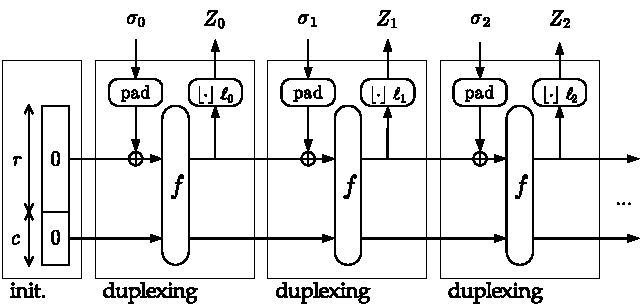
\includegraphics[width=0.8\textwidth]{img/Duplex.pdf}
\caption{The duplex construction $\mathbf{duplex}[f,\mathbf{pad},r]$ \cite{Bertoni2011_SpongeFunctions}}
\label{fig:Duplex}
\end{figure}
Figure~\ref{fig:Duplex} shows the duplex construction.
The $i$-th input is denoted $\sigma_i$ and the $i$-th output is denoted $Z_i$, which is truncated to $\ell_i$ bits.
Inputs are absorbed and processed at the same time that outputs are squeezed.
For a duplex object it is possible to have an empty input or to not request an output.
A \emph{blank call} is a call to $\mathbf{duplexing}$ for which no input is provided ($|\sigma_i| = 0$).
A \emph{mute call} is a call for which no output is requested ($\ell_i = 0$).

\subsection{Duplex for Authenticated Encryption}
Authenticated encryption is easily achieved using the duplex construction.
Figure~\ref{fig:DuplexAE_Expanded} shows such a use case.
First, we construct a duplex object $D$.
Then we absorb the key $K$ (or optionally $K||IV$) using one or more mute calls to $D.\mathbf{duplexing}$.
More that one mute call may be required if the length of the key exceeds the rate $r$.
We denote a header input to $D$ as $A$; these arbitrary length inputs are authenticated but not encrypted.
We denote a body input to $D$ as $B$; these arbitrary length inputs are both encrypted and authenticated.
$A$ inputs are absorbed using one or more mute calls to $D.\mathbf{duplexing}$.
$B$ inputs are absorbed in a similar fashion and then the keystream $Z$ is XORed with $B$ to produce the ciphertext $C$.
The tag $T$ is produced using a blank call to $D.\mathbf{duplexing}$ after all header and body inputs have been processed.

\begin{figure}[ht]
\centering
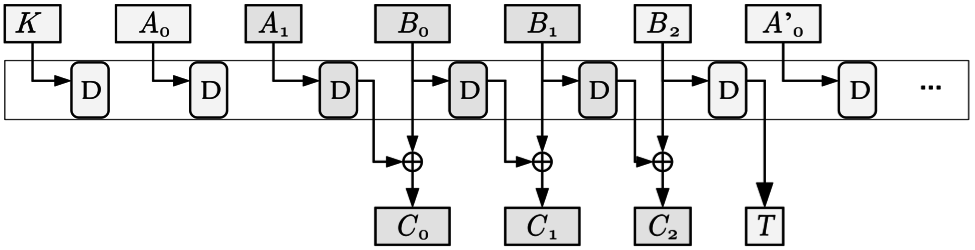
\includegraphics[width=0.8\textwidth]{img/DuplexAE_Expanded-BW.png}
\caption{The duplex construction as used for authenticated encryption \cite{Bertoni2010_DuplexingSlides}}
\label{fig:DuplexAE_Expanded}
\end{figure}

\begin{comment}
\begin{enumerate}
\item Easy to use
\item Single key required
\item Single-pass for encryption and authentication
\item Support for intermediate tags
\item Support for Additional Authenticated Data (AAD, or headers)
\item Secure against generic attacks
\item Ability to trade off speed and security by adjusting $r$
\end{enumerate}
\end{comment}

We note that the duplex construction may require \emph{domain separation}, a generic mechanism for eliminating output ambiguity.
For example, the simplest domain separation method consists of appending a \emph{frame bit} to the last block of every different input data type (e.g.\ key or message data).
This frame bit has the property that no two consecutive data types have the same frame bit value, meaning that one can easily identify where one data type ends and the next begins \cite{Bertoni2012_Duplexing}.

\subsection{Generic Security}
\label{sec:DuplexSecurity}
Any calls made to the duplex construction can be reduced to calls to the keyed sponge construction.
As a result, the security of the duplex construction depends only on its corresponding sponge construction.

The security of the sponge construction is based on the assumption that the underlying sponge function $f$ is secure.
That is, if $f$ is computationally indistinguishable from random then so should be the sponge construction it is instantiated within.
Consequently, cryptographers designing a system based on the sponge construction need only be concerned with designing and cryptanalyzing a secure underlying function.
The sponge construction, when used properly, is said to be secure against \emph{generic attacks} -- attacks which do not exploit any specific properties of the underlying sponge function.
We call this the \emph{generic security} of the construction \cite{Bertoni2011_SpongeFunctions}.

The generic security of keyed constructions is higher than unkeyed.
For our purposes we are interested only in the security of the keyed sponge construction where a permutation is used for $f$. 
Jovanovic et.~al\ \cite{Jovanovic2014_Beyond} proved in 2014 that the generic security level of keyed sponge constructions is lower bounded by 
\begin{equation*}
\mathrm{min}(2^{(r+c)/2}, 2^c, 2^{|K|}).
\end{equation*} 


%-----------------------------------
% SECTION: Algorithm Specification
%-----------------------------------
\section{Algorithm Specification}
\label{sec:AlgorithmSpec}
Our authenticated encryption algorithm is based on a simplified duplex construction.
Padding and domain separation are assumed to be done at some higher level in the overall system if needed.
For this reason, it is sufficient to specify only the duplex parameters and the sponge function $f$.

%\begin{algorithm}
\caption*{\textbf{Algorithm} $f$ Round}
\label{alg:Algorithm}
\begin{algorithmic}
\Comment{Substitution Step}
\For{$x < 16$}
  \State $S[x] \gets Sbox(S[x])$
\EndFor
\If {$i > maxval$}
    \State $i \gets 0$
\Else 
    \State $blah$
\EndIf
\end{algorithmic}
\end{algorithm}



\subsection{Duplex Parameters}
We allow two key sizes: $128$ bits and $256$ bits.
Our construction uses a $512$-bit internal state, so we have $b = 512$.
The rate $r$ is $128$ bits for both key lengths, which means that the capacity $c$ is $384$.
Keeping the rate at a constant $128$ bits for both instantiations means that switching between key lengths is a trivial task.

The capacity $c = 384$ provides sufficient security against generic attacks for both $128$- and $256$-bit keys.
As explained in Section~\ref{sec:SpongeAndDuplex}, we know from \cite{Jovanovic2014_Beyond} that the generic security level is
\begin{equation*}
\mathrm{min}(2^{(r+c)/2}, 2^c, 2^{|K|}).
\end{equation*}
For a $128$-bit key, the generic security level is $2^{128}$.
For a $256$-bit key, the generic security level is $2^{256}$. 

\subsection{Permutation $f$}
Our underlying sponge function $f$ is a permutation and thus is invertible.
For compactness, we specify only the forward permutation here as the inverse is not required for practical purposes.

The permutation consists of a number of rounds.
Each round can be represented as the composition of several subfunctions or \emph{steps}: a substitution, a bitwise permutation, a mixing layer, and the addition of a round constant.

\subsubsection{Substitution Step}
The substitution step is a bricklayer permutation that uses $32$ identical, bijective $16 \times 16$ S-boxes.
This step is the main source of confusion within the permutation.
Furthermore, it is the only nonlinear step, as is typical with many substitution-based symmetric key algorithms \cite{Stinson2006_CTAP}.

To the best of our knowledge this is the first cryptosytem to use such large S-boxes.
We believe that, at the time of writing, the largest S-boxes used in the literature are the $8 \times 8$ bijective S-boxes used by the Advanced Encryption Standard (AES) \cite{Daemen2002_DesignOfRijndael}\cite{NIST2001_FIPS-197}.

Our S-box is an AES-inspired design taken directly from Wood's thesis on the subject \cite{Wood2013_SboxThesis}.
The primary reason for using this particular class of $16$-bit S-boxes is that they are efficiently implementable in hardware.
Rather than being based on a random mapping, they are based on multiplicative inversion in a finite field followed by an affine transformation.
This allows us to implement a circuit which performs the field operations rather than use the corresponding (and prohibitively large) look-up table.

This S-box is based on multiplicative inversion in $\gfsixteen / \left\langle p(x) \right\rangle$ where 
\begin{equation*}
p(x) = x^{16} + x^5 + x^3 + x + 1.
\end{equation*}
We represent an input to the S-box (and inverse S-box) as a $16$-bit column vector 
\begin{equation*}
x = 
\begin{pmatrix}
x_{15} & x_{14} & \ldots & x_1 & x_0
\end{pmatrix}^\mathrm{T},
\end{equation*}
where $x_{15}$ is the MSB.
Using this notation, the forward S-box function is given as
\begin{equation*}
\renewcommand{\arraystretch}{0.7} % Make it square
\mathbf{S}(x) = 
\begin{pmatrix}
0 & 0 & 1 & 0 & 0 & 0 & 0 & 1 & 0 & 0 & 1 & 1 & 1 & 1 & 1 & 0 \\
1 & 1 & 0 & 0 & 0 & 0 & 0 & 1 & 0 & 1 & 1 & 0 & 1 & 0 & 1 & 0 \\
1 & 1 & 0 & 0 & 1 & 0 & 1 & 1 & 0 & 1 & 0 & 1 & 0 & 0 & 1 & 1 \\
1 & 1 & 1 & 0 & 0 & 0 & 1 & 0 & 0 & 1 & 1 & 0 & 0 & 0 & 0 & 0 \\

1 & 1 & 0 & 0 & 0 & 1 & 1 & 0 & 0 & 1 & 1 & 1 & 1 & 0 & 1 & 1 \\
0 & 1 & 0 & 0 & 0 & 0 & 1 & 1 & 0 & 1 & 1 & 1 & 1 & 1 & 0 & 1 \\
0 & 0 & 1 & 0 & 1 & 0 & 1 & 0 & 1 & 1 & 0 & 0 & 1 & 1 & 0 & 0 \\
1 & 0 & 1 & 1 & 1 & 0 & 1 & 1 & 0 & 0 & 0 & 1 & 0 & 1 & 1 & 1 \\

0 & 1 & 0 & 0 & 0 & 0 & 0 & 0 & 1 & 0 & 0 & 1 & 1 & 1 & 0 & 1 \\
1 & 0 & 1 & 1 & 0 & 0 & 0 & 1 & 0 & 0 & 1 & 0 & 1 & 0 & 0 & 0 \\
1 & 0 & 1 & 0 & 0 & 1 & 1 & 1 & 0 & 0 & 1 & 1 & 0 & 1 & 0 & 0 \\
1 & 0 & 1 & 1 & 1 & 0 & 1 & 1 & 1 & 1 & 0 & 1 & 1 & 0 & 0 & 1 \\

1 & 0 & 1 & 0 & 0 & 1 & 0 & 1 & 1 & 0 & 0 & 1 & 0 & 0 & 0 & 1 \\
0 & 1 & 0 & 0 & 0 & 1 & 1 & 1 & 1 & 0 & 0 & 0 & 0 & 0 & 0 & 1 \\
1 & 0 & 0 & 0 & 1 & 1 & 0 & 1 & 0 & 1 & 1 & 1 & 1 & 0 & 0 & 0 \\
1 & 1 & 0 & 1 & 0 & 1 & 1 & 0 & 1 & 0 & 0 & 1 & 1 & 0 & 0 & 0 \\
\end{pmatrix}
\begin{pmatrix}
x_{15} \\
x_{14} \\
x_{13} \\
x_{12} \\
x_{11} \\
x_{10} \\
x_{9} \\
x_{8} \\
x_{7} \\
x_{6} \\
x_{5} \\
x_{4} \\
x_{3} \\
x_{2} \\
x_{1} \\
x_{0} \\
\end{pmatrix}
^{-1}
\oplus
\begin{pmatrix}
0 \\
1 \\
0 \\
0 \\
0 \\
1 \\
0 \\
1 \\
1 \\
0 \\
1 \\
1 \\
0 \\
1 \\
1 \\
1 \\
\end{pmatrix}.
\end{equation*}

A hardware implementation for this particular S-box requires just $1238$ XOR gates and $144$ AND gates.

\subsubsection{Bitwise Permutation Step}
Bitwise permutations are easily implementable in hardware via a simple rerouting of wires.
Compared to a permutation on the words of the state, a bitwise permutation intuitively provides much better diffusion.
The bitwise permutation step is the main source of long-range (i.e.\ across the entire state) diffusion in the algorithm.

The bitwise permutation also helps maximize the minimum number of active S-boxes by being subject to certain constraints.
We use a permutation that satisfies the following properties:
\begin{enumerate}
\item All outputs of a given S-box go to $16$ different mixers
\item The permutation is a \emph{derangement}; it has no fixed points
\item High order; it does not repeat within the number of rounds
\item No low order bits; the order of any bit equals the order of the overall permutation
\item Easily definable by some affine function
\end{enumerate}
There is obviously no cryptographic significance to how ``easy'' it is to express a bitwise permutation.
This is merely to cut down on the search space and to avoid having to provide a table with $512$ entries to express the permutation.
The \emph{order} of a bitwise permutation is the number of times it must be applied before it ends up in its original orientation.
A particular bit in a bitwise permutation also has the notion of order and a bit of low order is one that returns to its original position before the entire permutation begins to cycle.
If a bit has order zero, it is unaffected by the bitwise permutation and is called a \emph{fixed point}.

We chose the following permutation to use for our algorithm since it is the first function to satisfy all properties:
\begin{equation*}
\pi(x) = 31x + 15 \bmod{512}
\end{equation*}
This bitwise permutation has order $32$.
For a complete listing of all bitwise permutations that satisfy our requirements, refer to Appendix~\ref{appx:BitwisePermutations}.

\subsubsection{Mix Step}
The purpose of the mix step is to provide local diffusion (i.e.\ across two words) and increase the linear and differential branch numbers of a round from two to three.
We use a mixer based on multiplication by a $2 \times 2$ matrix in \gfsixteen modulo the irreducible polynomial
\begin{equation*}
p(x) = x^{16} + x^5 + x^3 + x^2 + 1.
\end{equation*}
The mixer takes two words $A$ and $B$ as input and produces outputs $A'$ and $B'$ as follows:
\begin{equation*}
\begin{pmatrix}
A' \\ B'
\end{pmatrix}
=
\begin{pmatrix}
1 & x \\ x & x + 1
\end{pmatrix}
\begin{pmatrix}
A \\ B
\end{pmatrix}
\end{equation*}
The MSB of each word is taken as the leftmost bit and is represented by $x^{15}$. 

The forward mixer is efficiently implementable in hardware.
Figure~\ref{fig:MixerMatrix} shows how this matrix multiplication is implemented.
The $x*$ operation is a multiplication by $x$ in \gfsixteen.
Its implementation, which is shown in Figure~\ref{fig:xTimes}, is very simple. 

\begin{figure}[ht]
\centering
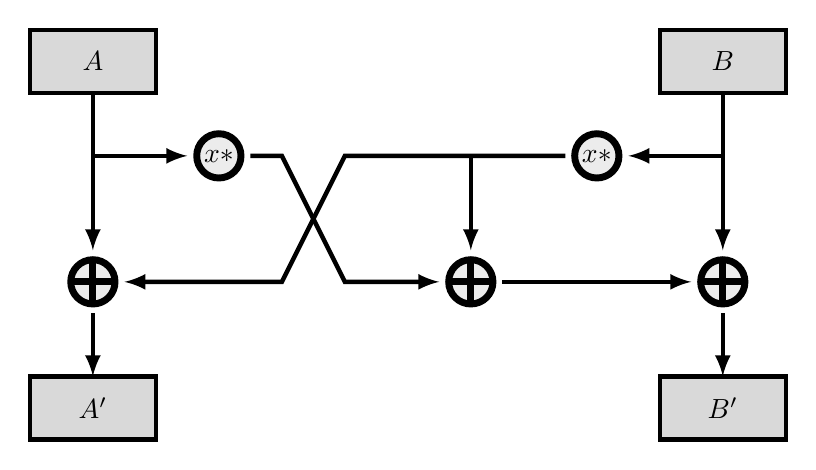
\begin{tikzpicture}[xscale=0.8,yscale=0.8,>=latex,ultra thick]
% Reference grid (temporary)
%\draw[help lines] (0,0) grid (16,16);

% Inputs
\draw[fill=gray!30] (0,15) rectangle (2,14) node[midway] {$A$};
\draw[fill=gray!30] (10,15) rectangle (12,14) node[midway] {$B$};

\draw[->] (1,14) to (1, 11.5);
\draw[->] (1,13) to (2.5, 13);

\draw[->] (11,14) to (11, 11.5);
\draw[->] (11,13) to (9.5, 13); 

\drawxTimes{3}{13}
\drawxTimes{9}{13}

\drawXOR{1}{11}
\drawXOR{11}{11}
\drawXOR{7}{11}

\draw[->] (3.5,13) to (4,13) to (5,11) to (6.5,11);
\draw[->] (8.5,13) to (5,13) to (4,11) to (1.5,11); 
\draw[->] (7,13) to (7,11.5);
\draw[->] (7.5,11) to (10.5,11);

\draw[->] (1,10.5) to (1,9.5);
\draw[->] (11,10.5) to (11,9.5);

% Outputs
\draw[fill=gray!30] (0,9.5) rectangle (2,8.5) node[midway] {$A'$};
\draw[fill=gray!30] (10,9.5) rectangle (12,8.5) node[midway] {$B'$};

\end{tikzpicture}

\caption{Hardware implementation of the forward mixer function.}
\label{fig:MixerMatrix}
\end{figure}

\begin{figure}[ht]
\centering
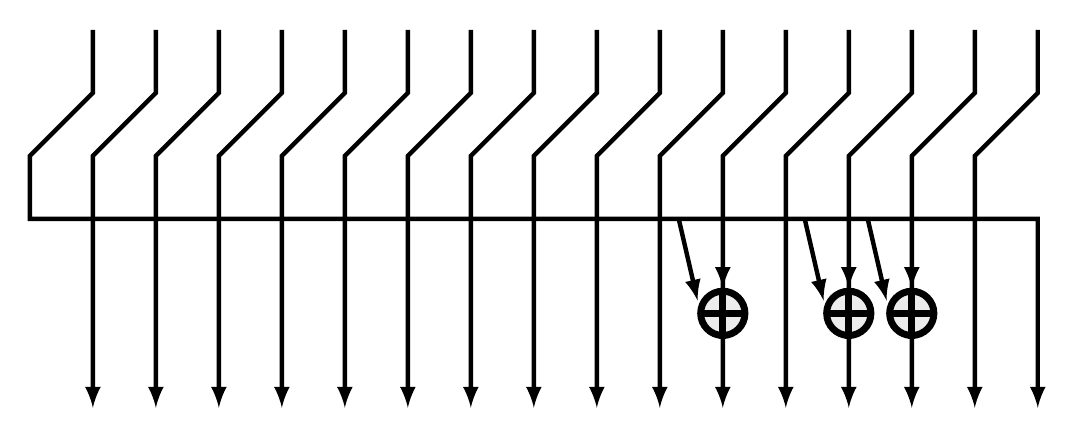
\begin{tikzpicture}[xscale=0.8,yscale=0.8,>=latex,ultra thick]
% Reference grid (temporary)
%\draw[help lines] (0,0) grid (24,24);

\draw[->] (1,24) to (1,23) to (0,22) to (0, 21)
    to (16, 21) to (16, 18);
\foreach \i in {2,...,16} {
    \draw[->] (\i,24) to (\i,23) to (\i-1,22) to (\i-1, 18);
}
\draw[->] (10.3,21) to (10.6,19.7);
\draw[->] (11,21) to (11,19.9);
\drawXOR{11}{19.5}
\draw[->] (12.3,21) to (12.6,19.7);
\draw[->] (13,21) to (13,19.9);
\drawXOR{13}{19.5}
\draw[->] (13.3,21) to (13.6,19.7);
\draw[->] (14,21) to (14,19.9);
\drawXOR{14}{19.5}
\end{tikzpicture}

\caption{Hardware implementation of the $x*$ function. The leftmost bit is the MSB.}
\label{fig:xTimes}
\end{figure}

\subsubsection{Add Round Constant Step}
This step consists of adding a $512$-bit value to the state using bitwise XOR in order to disrupt symmetry and prevent slide attacks.
The round constant $RC_i$ for round $i$ is given by the formula
\begin{equation*}
RC_i = \mathbf{SHA3\textbf{-}512}(\mathbf{ASCII}(i)),
\end{equation*}
where $\mathbf{ASCII}(i)$ is a function that provides the one or two byte ASCII representation of $i$ and $\mathbf{SHA3\textbf{-}512}$ is the SHA-3 hash function that outputs a $512$-bit message digest. 

\subsection{Number of Rounds}
This algorithm uses $10$ rounds for a $128$-bit key and $16$ rounds for a $256$-bit key.
The number of rounds is determined, as is typical with block ciphers and permutations, by calculating the number needed for resistance to linear and differential cryptanalysis and adding some buffer to increase the security margin. 
For a more in-depth treatment, refer to Section~\ref{sec:Cryptanalysis}.

\subsection{Customization}
While a specific instantiation is specified here, our algorithm is highly customizable within our security margin.
This could be useful in the case that different users want unique, proprietary algorithms.
We list several possible customizations here.

\subsubsection{State Initialization}
In the given specification, the inner state (like the outer state) is initialized to zero.
This is not a requirement; indeed, the inner state could be initialized to any $384$-bit value.
Each user could generate their own unique value to set during the initialization phase.
This happens before the first mute calls that absorb the key.

\subsubsection{S-boxes}
The AES-inspired S-box used here is efficiently implementable in hardware.
There are certainly many other cryptographically secure $16$-bit S-boxes, but randomly generated ones may not be suitable for hardware implementation due to size constraints.
This is an area for further research.
Still, several other AES-like $16$-bit S-boxes are presented in \cite{Wood2013_SboxThesis}.
Any new S-box introduced into the algorithm shall be analyzed to determine its linear and differential characteristics and the number of rounds should be adjusted accordingly if necessary.
This analysis can easily be performed using the tools mentioned in Section~\ref{sec:Cryptanalysis}.

\subsubsection{Bitwise Permutations}
The bitwise permutation provided in this algorithm specification is one of many that satisfies the constraints we impose.
We provide all suitable bitwise permutations in Appendix~\ref{appx:BitwisePermutations}.
Users may select any of these without need for further cryptanalysis.

\subsubsection{Mixers}
Our mixer is based on a specific $2 \times 2$ matrix multiplication in \gfsixteen modulo a specific irreducible polynomial $p(x)$.
Many matrices are expected to satisfy the constraints that we impose.
These constraints are:
\begin{enumerate}
\item The $2 \times 2$ matrix should be invertible in $\gfsixteen /\left\langle p(x) \right\rangle$
\item The matrix should have differential and linear branch number equal to three (the maximum possible)
\end{enumerate}
Like the addition of a new S-box, any new matrix introduced to the algorithm should be analyzed to ensure it meets these constraints.
This analysis can also easily be performed using the tools mentioned in Section~\ref{sec:Cryptanalysis}.

\subsubsection{Round Constants}
The round constants presented here are based on SHA-3 hash values.
However, they could be any values that satisfy the following constraints.
Round constants should be:
\begin{enumerate}
\item Unique for each round; to prevent against slide attacks
\item Random, pseudorandom, or highly asymmetric; to reduce symmetry in the state
\end{enumerate}
The round constants are not expected to have any cryptographic significance outside of this.
Different users can generate their own unique set of round constants without difficulty.


%------------------------------
% SECTION: Preliminary Cryptanalysis
%------------------------------
\section{Preliminary Cryptanalysis}
\label{sec:Cryptanalysis}
The duplex construction has been shown to be secure against generic attacks by the \Keccak team \cite{Bertoni2011_SpongeFunctions}.
Therefore it is sufficient for us to assess only the security of the underlying sponge permutation $f$.

We provide an overview of our preliminary cryptanalysis here.
Emphasis is placed on the most general and prevalent forms of attacks.
Resistance against these techniques should result in resistance against many other less general techniques.
Our aim is to provide intuitive explanations of prevalent methods and simply explain why our permutation should be resistant.
Further cryptanalysis, as with all cryptosystems, is always welcome for future work.

%------------------------------
% Differential Cryptanalysis
%------------------------------
\subsection{Differential Cryptanalysis}
Differential cryptanalysis was publicly introduced by Biham and Shamir in 1991 in their landmark paper on the subject \cite{Biham1991_Differential}.
Since then, it has been applied with varying degrees of success to a great number of cryptosystems.
As such, it is a fundamental requirement of symmetric key cryptosystem design to prove resistance to differential cryptanalysis.

\subsubsection{Overview}
The goal of differential cryptanalysis is to exploit non-random behavior of a system (in our case, a permutation) with regard to the propagation of differences.
A \emph{difference}, denoted $\Delta X$, is the bitwise XOR (for our case) of two bitstrings. For example,
\begin{equation*}
\Delta X = X' \oplus X''
\end{equation*}
is the difference between bitstrings $X'$ and $X''$.
For differential cryptanalysis, a difference $\Delta X$ is fed through a system and a resulting difference $\Delta Y$ is obtained.
The pair of these two related differences is called a \emph{differential} and is denoted $(\Delta X,\Delta Y)$.

Differentials occur with some associated probability.
For an ideal system the probability of a given differential is $1/2^n$ where $n$ is the length of the bitstrings involved.
A system is said to exhibit non-random behavior if the magnitude of the probability $p_D$ for some differential $(\Delta X, \Delta Y)$ is much greater than the ideal value.
This information could be used to mount an attack on the system \cite{Heys2002_Tutorial}.

To launch an effective attack, a cryptanalyst first has to focus on the S-boxes.
The S-boxes are analyzed to determine their maximum differential probabilities.

A \emph{differential trail} or \emph{characteristic} is the propagation of non-zero differentials throughout a system (i.e.\ across rounds).
A \emph{differentially active} S-box is an S-box that has a non-zero difference at its input during an attack; it is part of a differential trail.

Proving resistance against differential cryptanalysis for a substitution-permutation network requires computing a lower bound on the minimum number of active S-boxes across some number of rounds.
The more active S-boxes there are, the less likely an attack is to succeed since exponentially more chosen plaintexts will be needed for additional each active S-box.
The \emph{branch number} of an operation is of particular importance here. 
It can be simply defined as the minimum number of active S-boxes across just two rounds of a system (e.g.\ our permutation).
The technique of maximizing the branch number of a round is known as the \emph{wide trail design strategy}.
It is the main design strategy behind AES, which has a round branch number of five \cite{Daemen2001_WideTrail}\cite{Daemen2002_DesignOfRijndael}.

The number of plaintext/ciphertext pairs required to mount a successful differential attack should exceed the number required for a brute force attack.
As the differential probability reduces across rounds, more pairs are required for a successful attack.
We loosely refer to the number of pairs required as the \emph{complexity} of the differential attack.
The number of rounds is increased until this complexity exceeds that of a brute force method.

\subsubsection{Algorithm Resistance}
To determine the resistance of our algorithm to differential cryptanalysis, we first have to determine the maximum differential probability of our S-box.
We determined this value to be $p_{D,max} = 2^{-14}$ using an S-box evaluation program called \texttt{Eval16BitSbox} \cite{Kaminsky2014_BlockCipherAnalysis} written with Kaminsky's Parallel Java 2 library \cite{Kaminsky2014_PJ2}.

Next, it is necessary to determine the branch number of a round.
For this, we only need to analyze the mixer. 
We purposefully designed a mixer with differential branch number equal to three, meaning that minimally three S-boxes will be differentially active between two rounds.
This is in fact the maximum achievable branch number for a transformation defined by multiplication by a $2 \times 2$ matrix.
To verify this, we used a SAT solver called CryptoMiniSat \cite{Soos2014_CryptoMiniSat}.
This SAT solver takes as input a Boolean equation in conjunctive normal form (CNF) and determines if it is \emph{satisfiable}; that is, if it can ever produce an output of `$1$' for any set of input values.
Our CNFs were generated using Kaminsky's \texttt{SatProblem} Java class \cite{Kaminsky2014_BlockCipherAnalysis}.

The CNFs generated are unsatisfiable if and only if the mixer has differential branch number equal to three since it answers the following question: \emph{is it possible to have a difference in only one input and only one output?}
Through SAT solver analysis we determined that this is not possible for our mixer; that is, if there is a non-zero difference in only one input, there must be a non-zero difference in each output.
In the event that there is a difference in both inputs, there may be a difference in only one output.
This still leads to a differential branch number of three since two S-boxes must have been active in the previous round to lead to those two input differences.
The probability of a difference in either output is $p_{D,out} = 2^{-15}$.

With all of this information, it is possible to calculate the number of rounds needed for resistance to differential attacks.
The worst-case probability of successfully propagating a difference over two rounds is given by
\begin{equation*}
(p_{D,max})^{\mathcal{B}_D} \cdot p_{D,out},
\end{equation*}
where $\mathcal{B}_D = 3$ is the differential branch number.
From this we constructed Table~\ref{tab:DifferentialProbabilities}, which shows the worst-case differential probabilities for higher numbers of rounds.
\begin{table}[ht]
\centering
\begin{tabular}{c|c}
Rounds & Worse Case Differential Probability \\
\hline
$2$  & $2^{-57}$  \\
$4$  & $2^{-114}$ \\
$6$  & $2^{-171}$ \\
$8$  & $2^{-228}$ \\
$10$ & $2^{-285}$ \\
$12$ & $2^{-342}$ \\
$14$ & $2^{-399}$ \\
$16$ & $2^{-456}$ \\
\end{tabular}
\caption{Worst case differential probabilities over increasing rounds}
\label{tab:DifferentialProbabilities}
\end{table}

Therefore the complexity of a differential attack exceeds the complexity of a brute force search of a $128$-bit keyspace at six rounds.
To increase our security margin significantly, we require $10$ rounds for a $128$-bit key.
For a $256$-bit key, $16$ rounds are required to achieve a similar security margin.

%------------------------------
% Linear Cryptanalysis
%------------------------------
\subsection{Linear Cryptanalysis}
Linear Cryptanalysis was first introduced by Matsui in 1993 in his landmark paper, \cite{Matsui1993_Linear}.
As with differential cryptanalysis, it is a fundamental requirement of symmetric key cryptosystem design to prove resistance against linear attacks.

\subsubsection{Overview}
Linear cryptanalysis is surprisingly similar to differential cryptanalysis in many ways. 
However, for linear cryptanalysis we are concerned with estimating the behavior of a system using linear expressions rather than highly probable differential characteristics.
As with differential cryptanalysis, the first step is to analyze the S-boxes involved in the substitution-permutation network.
An S-box, by definition, should be highly nonlinear to provide sufficient confusion. 
However, it is possible to uncover linear approximations of S-box outputs that occur with high (or low) probability.
We can represent our S-box as a vectorial Boolean function 
\begin{equation*}
S \from \Ztwo^{16} \to \Ztwo^{16}
\end{equation*}
in which the input $X$ and output $Y$ are represented as row vectors, e.g.\
\begin{equation*}
X = \begin{pmatrix}X_1 & X_2 & ... & X_{15} & X_{16} \end{pmatrix},
\end{equation*}
where $X_i \in \Ztwo$.
Favoring typical convention found in the literature, $X_1$ is the MSB \cite{Heys2002_Tutorial}.
This notation allows us to easily represent linear approximations in the form
\begin{equation*}
\left( \bigoplus\limits_{i=1}^{16} X_i \right) = \left( \bigoplus\limits_{i=1}^{16} Y_i \right).
\end{equation*}

The ideal \emph{linear probability} $p$ that such an approximation holds true is exactly equal to 1/2.
We are concerned with deviations from this ideal probability, known as the \emph{linear bias}, $\epsilon$. 
Clearly, $\epsilon = p - 1/2$.
We found the maximum linear bias of our particular S-box to be $\epsilon_{L,max} = 2^{-8}$ using the same program as previously described.

The \emph{linear branch number} $\mathcal{B}_L$ is the minimum number of linearly active S-boxes across two rounds of our permutation.
As with differential cryptanalysis, it depends solely on our mixer.

\subsubsection{Algorithm Resistance}
Recall that we have verified via SAT solver analysis that the differential branch number of our mixer is three.
In \cite{Daemen2002_DesignOfRijndael}, Daemen and Rijmen prove the following result: the linear branch number of a linear transformation specified by multiplication by a matrix $M$ is equal to the differential branch number of the linear transformation specified by the transpose of that matrix.
Therefore, a sufficient condition for the differential and linear branch numbers to be equal is that the matrix is symmetric.
Our matrix is symmetric, and therefore we know $\mathcal{B}_D = \mathcal{B}_L$ without the need for further analysis.

The final step to prove the resistance of our algorithm against linear cryptanalysis involves determining the linear bias of two complete rounds of our permutation.
To combine linear biases, we use Matsui's Piling-Up Lemma from \cite{Matsui1993_Linear}:
\begin{equation*}
\epsilon = 2^{n-1} \prod\limits_{i = 1}^n \epsilon_i,
\end{equation*}
where $n = 3$ is the number of linearly active S-boxes across two rounds and $\epsilon_i = \epsilon_{L,max} = 2^{-8}$ is the worst case linear bias of those S-boxes.
Note that we need not consider the mixer since, being a linear function, it must have a maximum linear probability $p_{mix} = 1$, corresponding to a maximum bias of $\epsilon_{mix} = 1/2$. This gets cancelled out.
Also from Matsui's paper, we know that the number of plaintext/ciphertext pairs (again referred to loosely as the \emph{complexity}) needed to exploit the overall bias $\epsilon$ is approximately $\epsilon^{-2}$.
Using this information, we constructed Table~\ref{tab:LinearBiases}.

\begin{table}[ht]
\centering
\begin{tabular}{c|c|c}
Rounds & Worst Case Linear Bias & PT/CT Pairs Required \\
\hline
$2$  & $2^{-22}$  & $2^{44}$  \\
$4$  & $2^{-44}$  & $2^{88}$  \\
$6$  & $2^{-66}$  & $2^{132}$ \\
$8$  & $2^{-88}$  & $2^{176}$ \\
$10$ & $2^{-110}$ & $2^{220}$ \\
$12$ & $2^{-132}$ & $2^{264}$ \\
$14$ & $2^{-154}$ & $2^{308}$ \\
$16$ & $2^{-176}$ & $2^{352}$ \\
\end{tabular}
\caption{Worst case linear biases and linear attack complexities over increasing rounds}
\label{tab:LinearBiases}
\end{table}

Therefore the complexity of a linear attack exceeds the complexity of a brute force search of a $128$-bit keyspace at six rounds.
To increase our security margin significantly, we require $10$ rounds for a $128$-bit key.
For a $256$-bit key, $16$ rounds are required to achieve a similar security margin.

\subsection{Algebraic Attacks}
Differential and linear cryptanalysis take a probabilistic approach to estimating the behavior of a system.
In contrast, algebraic attacks take a deterministic approach in that they aim to find mathematical models of a system that hold with unity probability.
For example, in 2001 Ferguson et~al.\ \cite{Ferguson2001_AlgebraicRijndael} introduced an elegant and complete algebraic representation of AES.
The ability to create such a simple mathematical representation of the cipher initially raised alarm throughout the cryptographic community.
However, the security of AES seems to be uncompromised since we believe it is far too difficult to solve such an algebraic system - the algebraic complexity of the AES S-box is too high.

Until there is reason to believe otherwise, it seems that these algebraic attacks would be highly ineffective against our permutation.
Even if there were a practical algebraic attack demonstrated on AES, which all literature indicates as highly implausible right now, the much larger size of our S-box and therefore the much higher algebraic complexity (see \cite{Wood2013_SboxThesis}) leads us to conjecture that our permutation would still be resistant.


%%%%%%%%%%%%%%%%%%%%%%%%%%%%%%%%%%%%
% Section: Conclusions \& Future Work
%%%%%%%%%%%%%%%%%%%%%%%%%%%%%%%%%%%%
\section{Conclusions \& Future Work}
\begin{frame}
\frametitle{Conclusions}
\begin{itemize}
  \item AE is an extremely popular and important topic right now
  \item We provide our own novel solution
  \item Provides nearly all desired properties of AE:
  \begin{itemize}
    \item Easy to use
    \item Single key, single pass
    \item Header support
    \item Intermediate MACs
  \end{itemize}
  \item \textbf{Easily} customizable on per-user / application basis
\end{itemize}
\end{frame}

\begin{frame}
\frametitle{Future Work}
\begin{itemize}
  \item Actual hardware implementation
  \item More cryptanalysis - always
  \item Complete analysis of all 16-bit S-boxes by Wood
  \begin{itemize}
    \item Easier customization
  \end{itemize}
  \item Find larger matrices with maximum branch number (MDS matrices)
  \begin{itemize}
    \item Decrease rounds
  \end{itemize}
  \item Much more!
\end{itemize} 
\end{frame}



\begin{frame}
\frametitle{Questions}
\begin{center}
\Huge ?
\end{center}
\end{frame}

%------------------------------------------------
% BIBLIOGRAPHY
%------------------------------------------------
\section*{Bibliography}
\begin{frame}[allowframebreaks]
\frametitle{Bibliography}
\tiny
\bibliographystyle{plain}
\bibliography{defense}
\end{frame}

\end{document}

